

%%%%% MOTIVATION & INTRODUCTION
\frame{
\begin{tikzpicture}[remember picture,overlay]
\fill[blue1]
(current page.north west) rectangle ([xshift=0.55\paperwidth,yshift=0.27\paperheight]current page.west|-{pic cs:end});
\end{tikzpicture}
\begin{textblock}{0.55}(0.02,0.03)
	\textcolor{white}{							
	\Large{X-ray radiography of granular systems \\
		-- particle densities and dynamics}
	}
\end{textblock}

\begin{textblock}{0.25}(0.1,0.35)
\only<1>{

\includegraphics[width=\textwidth]{Sources/motivation/setup-fluidized_bed_sedimented.pdf}}
\only<2>{

\includegraphics[width=\textwidth]{Sources/motivation/setup-fluidized_bed_expanded.pdf}}
\end{textblock}

\begin{textblock}{0.55}(0.02,0.2)
\visible<3->{
	Fluidized bed\\[0.5cm]
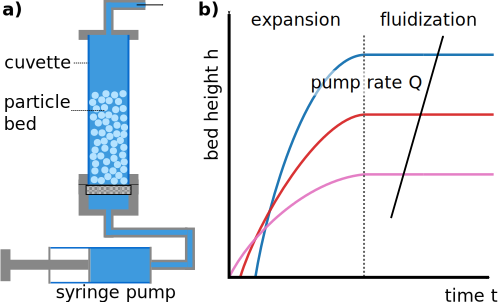
\includegraphics[width=\textwidth]{Sources/motivation/setup-fluidized_bed_final.pdf}}
\end{textblock}

\begin{textblock}{0.4}(0.6,0.02)
\visible<4->{
\begin{center}

\includegraphics[width=0.7\textwidth]{Sources/motivation/linked_together.pdf}
\end{center}
}
\end{textblock}

\begin{textblock}{0.38}(0.6,0.5)
\visible<5->{
	\begin{minipage}[c]{0.2\textwidth}
	\includegraphics[width=\textwidth]{Sources/motivation/wikipedia_hd.png}
	\end{minipage}
	\hfill
	\begin{minipage}[c]{0.75\textwidth}
	{\large Fluidized bed reactor}
	\end{minipage}
	\vfill
	\vspace{0.2cm}
	\begin{minipage}[b]{.9\textwidth}
	"\textbf{Lack of understanding:}\\
	It is very difficult to predict and calculate the \textcolor{red}{complex mass} [...] \textcolor{red}{flows} within the bed."
	\end{minipage}
}
\end{textblock}

\note{
athermal
frictional
dissipative -- permanent \textit{heating} necessary
jamming transition

}
}

%% OPAQUE
\frame{
	\begin{tikzpicture}[remember picture,overlay]
	\fill[blue1]
	(current page.north west) rectangle ([xshift=12.cm,yshift=-10.cm]current page.east|-{pic cs:end});
	\end{tikzpicture}
	\frametitle{\textcolor{white}{Particulate flows are \textbf{opaque}}}
	\begin{textblock}{0.9}(0.05,0.05)
		\centering
		\Large{
			\textcolor{white}{Particulate flows are \textbf{opaque}}}
	\end{textblock}

	\begin{textblock}{0.5}(0.0,0.15)
		\centering
		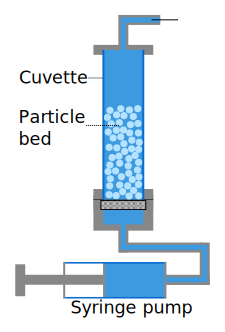
\includegraphics[height=0.75\textheight]{Sources/motivation/setup-fluidized_bed_left.pdf}
	\end{textblock}

	\begin{textblock}{0.5}(0.5,0.15)
		\centering
		\movie[height=0.75\textheight,loop]
		{\includegraphics[height=0.75\textheight]{Sources/motivation/video_welm_paetzold.png}}	
		{Sources/motivation/video_welm_paetzold.avi}
		
		\textcolor{white}{\footnotesize Master thesis Welm Pätzold}
	\end{textblock}

}


%% X-RAY RADIOGRAPHY
\frame{
\begin{tikzpicture}[remember picture,overlay]
\fill[blue1]
(current page.north west) rectangle ([xshift=0.28\paperwidth,yshift=0.33\paperheight]current page.west|-{pic cs:end});
\end{tikzpicture}

\begin{textblock}{0.5}(0.02,0.03)
	\textcolor{white}{
		\Large X-ray radiography}
\end{textblock}

\begin{textblock}{0.7}(0.02,0.05)
	\centering
	\only<1>{
	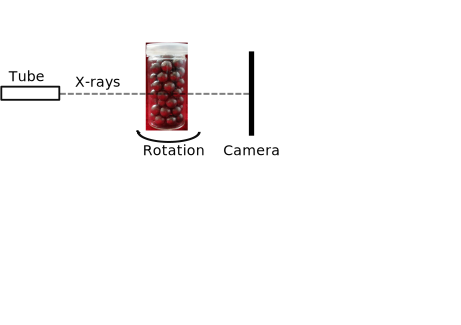
\includegraphics[width=\textwidth]{Sources/motivation/x-ray_setup_use0.pdf}}
	\visible<2->{
	\includegraphics[width=\textwidth]{Sources/motivation/x-ray_setup_use.pdf}}
\end{textblock}

%% Video of Projections
\begin{textblock}{0.22}(0.45,0.05)
	\visible<1->{
	\centering
	Radiogram\\
	\fbox{
	\movie[width =\textwidth,loop]
	{\includegraphics[width=\textwidth]{Sources/motivation/Projection0000.png}}
	{Sources/motivation/Projections360degree_fast.avi}}}
\end{textblock}

\begin{textblock}{0.28}(0.7,0.25)
	\visible<1->{
	2D projections of 3D object\\
	\textcolor{blue1}{Short} acquisition time}
\end{textblock}

% Video of Tomography
\begin{textblock}{0.2}(0.05,0.48)
	\visible<2->{
	\centering
	Tomogram\\
	\movie[width =\textwidth,loop]
	{\includegraphics[width=\textwidth]{Sources/motivation/Images_tomo_movie0000.png}}
	{Sources/motivation/tomogram_360degree.avi}}
\end{textblock}

\begin{textblock}{0.5}(0.27,0.8)
	\visible<2->{
	Full 3D information\\
	\textcolor{red}{Long} acquisition time\\
	$\rightarrow$ static objects}
\end{textblock}

% Video of Tomography
\begin{textblock}{0.23}(0.72,0.5)
	\visible<3->{
		\centering
		\textcolor{blue1}{Dynamic} system\\
		\movie[width =\textwidth,loop]
		{\includegraphics[width=\textwidth]{Sources/motivation/10000mul_per_min_0000.png}}
		{Sources/motivation/10000mul_per_min_original.avi}}
\end{textblock}
}


